\documentclass[border=0.1cm]{standalone}
\usepackage{tikz}
\usetikzlibrary{arrows, arrows.meta}

\tikzset{
    barbarrow/.style={ % style that just defines the arrow tip
        %>={Straight Barb[left,length=5pt,width=5pt]},
        >={Triangle[left,length=5pt,width=5pt]},
        double,
        semithick,
        <->
    },
    whites/.style={
        thick, 
        color=white
    }
}
\definecolor{light-gray}{gray}{0.9}
\definecolor{pcolor}{rgb}{0.21, 0.27, 0.31}

\begin{document}
    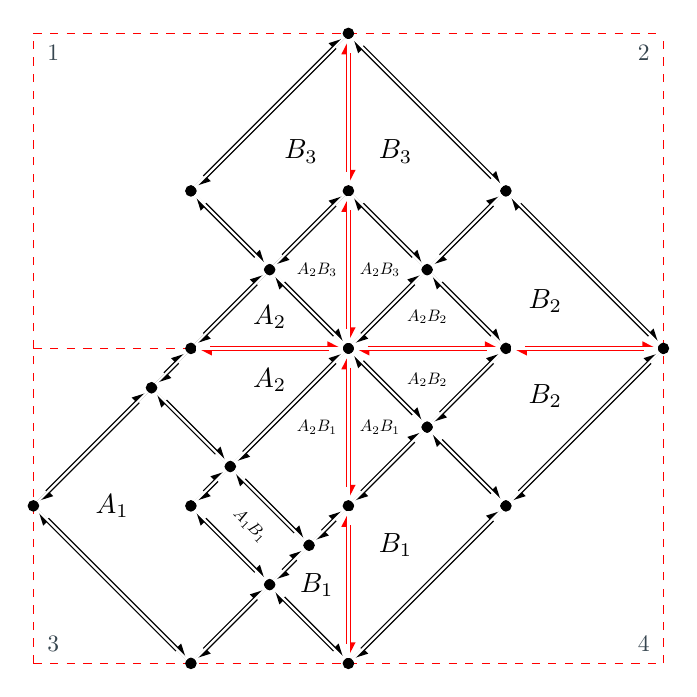
\begin{tikzpicture}
        \tikzstyle{node1}=[draw,scale=0.4,shape=circle,color=black,fill=black]
        \tikzstyle{node2}=[draw,scale=0.4,shape=circle,color=red,fill=red]
        %\draw[color=light-gray, style=dashed] (0,0) grid (8,8);
        \draw[color=red, style=dashed, step=4] (0,0) grid (8,8);
        \node[node1] (A) at (0,2) {};    \node[node1] (C) at (2,0) {};
        \node[node1] (D) at (2,2) {};    \node[node1] (E) at (2,4) {};
        \node[node1] (F) at (2,6) {};    \node[node1] (G) at (3,1) {};
        \node[node1] (H) at (2.5,2.5) {};    \node[node1] (I) at (3,5) {};
        \node[node1] (J) at (4,0) {};    \node[node1] (K) at (4,2) {};
        \node[node1] (L) at (4,4) {};    \node[node1] (M) at (4,6) {};
        \node[node1] (N) at (4,8) {};    \node[node1] (O) at (5,3) {};
        \node[node1] (P) at (5,5) {};    \node[node1] (Q) at (6,2) {};
        \node[node1] (R) at (6,4) {};    \node[node1] (S) at (6,6) {};
        \node[node1] (T) at (8,4) {};

        \node[node1] (X) at (1.5,3.5) {};
        \node[node1] (Y) at (3.5,1.5) {};


        \node at (1,2)      {$A_1$};
        \node at (6.5,4.6)  {$B_2$};
        \node at (6.5,3.4)  {$B_2$};
        \node at (3.4,6.5)  {$B_3$};
        \node at (4.6,6.5)  {$B_3$};
        \node at (4.6,1.5)  {$B_1$};
        \node at (3.6,1)    {$B_1$};
        \node at (3,4.4)    {$A_2$};
        \node at (3,3.6)    {$A_2$};
        \node[scale=0.6, rotate=-45] at (2.75,1.75)              {$A_1B_1$};
        \node[scale=0.6] at (3.6,3) {$A_2B_1$};
        \node[scale=0.6] at (4.4,3) {$A_2B_1$};
        \node[scale=0.6] at (5,4.4) {$A_2B_2$};
        \node[scale=0.6] at (5,3.6) {$A_2B_2$};
        \node[scale=0.6] at (3.6,5) {$A_2B_3$};
        \node[scale=0.6] at (4.4,5) {$A_2B_3$};

        \draw[barbarrow] (A) -- (X);
        \draw[barbarrow] (X) -- (E);
        \draw[barbarrow] (G) -- (Y);
        \draw[barbarrow] (Y) -- (K);

        \draw[barbarrow] (A) -- (C);%\draw[barbarrow] (A) -- (E);
        \draw[barbarrow] (C) -- (G);\draw[barbarrow] (D) -- (G);
        \draw[barbarrow] (D) -- (H);\draw[barbarrow] (X) -- (H);
        \draw[barbarrow] (E) -- (I);\draw[barbarrow] (F) -- (I);
        \draw[barbarrow] (F) -- (N);\draw[barbarrow] (G) -- (J);
        \draw[barbarrow] (H) -- (L);\draw[barbarrow] (I) -- (L);
        \draw[barbarrow] (I) -- (M);\draw[barbarrow] (J) -- (Q);
        %\draw[barbarrow] (G) -- (K);
        \draw[barbarrow] (H) -- (Y);
        \draw[barbarrow] (K) -- (O);\draw[barbarrow] (L) -- (O);
        \draw[barbarrow] (L) -- (P);\draw[barbarrow] (M) -- (P);
        \draw[barbarrow] (N) -- (S);\draw[barbarrow] (O) -- (Q);
        \draw[barbarrow] (O) -- (R);\draw[barbarrow] (P) -- (R);
        \draw[barbarrow] (P) -- (S);\draw[barbarrow] (Q) -- (T);
        \draw[barbarrow] (S) -- (T);

        \draw[whites] (A) -- (X);
        \draw[whites] (X) -- (E);
        \draw[whites] (G) -- (Y);
        \draw[whites] (Y) -- (K);

        \draw[whites] (A) -- (C);%\draw[whites] (A) -- (E);
        \draw[whites] (C) -- (G);\draw[whites] (D) -- (G);
        \draw[whites] (D) -- (H);\draw[whites] (X) -- (H);
        \draw[whites] (E) -- (I);\draw[whites] (F) -- (I);
        \draw[whites] (F) -- (N);\draw[whites] (G) -- (J);
        \draw[whites] (H) -- (L);\draw[whites] (I) -- (L);
        \draw[whites] (I) -- (M);\draw[whites] (J) -- (Q);
        %\draw[whites] (G) -- (K);
        \draw[whites] (H) -- (Y);
        \draw[whites] (K) -- (O);\draw[whites] (L) -- (O);
        \draw[whites] (L) -- (P);\draw[whites] (M) -- (P);
        \draw[whites] (N) -- (S);\draw[whites] (O) -- (Q);
        \draw[whites] (O) -- (R);\draw[whites] (P) -- (R);
        \draw[whites] (P) -- (S);\draw[whites] (Q) -- (T);
        \draw[whites] (S) -- (T);

        \draw[barbarrow, color=red] (R) -- (T);\draw[whites] (R) -- (T);
        \draw[barbarrow, color=red] (M) -- (N);\draw[whites] (M) -- (N);
        \draw[barbarrow, color=red] (K) -- (J);\draw[whites] (K) -- (J);
        \draw[barbarrow, color=red] (L) -- (E);\draw[whites] (L) -- (E);
        \draw[barbarrow, color=red] (L) -- (R);\draw[whites] (L) -- (R);
        \draw[barbarrow, color=red] (L) -- (M);\draw[whites] (L) -- (M);
        \draw[barbarrow, color=red] (L) -- (K);\draw[whites] (L) -- (K);

    \node[scale=0.85, color = pcolor] at (0.25, 7.75) {$1$};
    \node[scale=0.85, color = pcolor] at (7.75, 7.75) {$2$};
    \node[scale=0.85, color = pcolor] at (0.25, 0.25) {$3$};
    \node[scale=0.85, color = pcolor] at (7.75, 0.25) {$4$};
    \end{tikzpicture}
\end{document}
